\documentclass[12pt]{article}

%-- Packages, Environments, ...
%%%%%%%%%%%%%%%%%%%%%%%%%%%%%%%%%%%%%%%%%%%%%%%%%%%%%%%%%%%%
%2345678901234567890123456789012345678901234567890123456789012345678901234567890
%        1         2         3         4         5         6         7         8

\documentclass[letterpaper, 10 pt, conference]{ieeeconf}  % Comment this line out
                                                          % if you need a4paper
%\documentclass[a4paper, 10pt, conference]{ieeeconf}      % Use this line for a4
                                                          % paper

\IEEEoverridecommandlockouts                              % This command is only
                                                          % needed if you want to
                                                          % use the \thanks command
\overrideIEEEmargins
% See the \addtolength command later in the file to balance the column lengths
% on the last page of the document



% The following packages can be found on http:\\www.ctan.org
%\usepackage{graphics} % for pdf, bitmapped graphics files
%\usepackage{epsfig} % for postscript graphics files
%\usepackage{mathptmx} % assumes new font selection scheme installed
%\usepackage{times} % assumes new font selection scheme installed
%\usepackage{amsmath} % assumes amsmath package installed
%\usepackage{amssymb}  % assumes amsmath package installed
\usepackage{graphicx}
\usepackage{verbatim}
\usepackage{multirow}
\usepackage{rotating}
\usepackage{moreverb}                    % for boxedboxedverbatim
\usepackage{array}
\usepackage{fancyvrb}
\usepackage{multicol}
\usepackage{mdwlist}
\usepackage{enumerate}
%\usepackage{tikz-er2}


\newtheorem{defn}{Definition}

\newcommand{\class}[1] {\textit{#1}}
\newcommand{\const}[1] {$\mathit{#1}$}
\newcommand{\objvar}[1] {$\mathsf{#1}$}
\newcommand{\stvar}[1] {\textsf{#1}}
\newcommand{\op}[1] {\textsl{#1}}
\newcommand{\nil} {\textit{nil}\ }

\newcommand\T{\rule{0pt}{2.6ex}}
\newcommand\B{\rule[-1.2ex]{0pt}{0pt}}

%\definecolor{violetred}{cmyk}{0,0.85,0.31,0.18}
%\definecolor{darkblue}{cmyk}{1,1,0,0.45}
%\definecolor{lavenderblush4}{cmyk}{0,0.06,0.04,0.45}
%\definecolor{packergreen}{cmyk}{0.46,0,0.21,0.76}
%\definecolor{fuschia}{cmyk}{0,100,0,0}
%\definecolor{graycmyk}{cmyk}{0,0,0,0.74}
%
%\usetikzlibrary{calc,trees,positioning,arrows,chains,shapes.geometric,%
%    decorations.pathreplacing,decorations.pathmorphing,shapes,%
%    matrix,shapes.symbols,positioning,shadows}
%
%% styles for flowcharts
%
%\tikzstyle{every entity} = [top color=white, bottom color=blue!30,
%                            draw=blue!50!black!100, drop shadow]
%\tikzstyle{empty} = [top color=white, bottom color=white,
%                            draw=white]
%
%\tikzstyle{every weak entity} = [drop shadow={shadow xshift=.7ex,
%                                 shadow yshift=-.7ex}]
%\tikzstyle{every attribute} = [top color=white, bottom color=green!20,
%                               draw=green, node distance=1cm, drop shadow]
%\tikzstyle{ELLIPSE} = [draw, ellipse, top color=white, bottom color=green!20, draw=green, drop shadow]
%\tikzstyle{MainAttribute} = [draw, rectangle,top color=white, bottom color=red!20,
%                               draw=red, node distance=1cm, drop shadow]
%\tikzstyle{DATABASE} = [draw, rectangle, rounded corners,top color=white, bottom color=graycmyk!50, draw=graycmyk, inner sep=10pt, drop shadow={shadow xshift=.7ex, shadow yshift=-.7ex}]
%
%
%\tikzstyle{myarrow}=[->, >=stealth', thick, shorten <=2pt,shorten >=2pt]
%
%
%
%\tikzstyle{output} = [draw, rectangle, rounded corners,top color=white, bottom color=red!30, draw=red, inner sep=10pt, drop shadow={shadow xshift=.7ex, shadow yshift=-.7ex}]
%
%\tikzstyle{abstract}=[rectangle, draw=black, rounded corners, fill=blue!40, drop shadow,
%        text centered, anchor=north, text=white, text width=3cm]
%
%
%\newbox{\LegendOutput}
%\savebox{\LegendOutput}{
%    (\begin{tikzpicture}[]
%    \node[output] (2) {\hspace{5 mm}};
%    \end{tikzpicture}
%    )}


\newenvironment{mylisting}
{\begin{list}{}{\setlength{\leftmargin}{1em}}\item\small}
{\end{list}}

\newenvironment{mytinylisting}
{\begin{list}{}{\setlength{\leftmargin}{1em}}\item\tiny\bfseries}
{\end{list}}


\title{\LARGE \bf
Metrics and Test Methods for Industrial Kit Building
}

%\author{ \parbox{3 in}{\centering Stephen Balakirsky\\
%         Intelligent Systems Division\\
%         National Institute of Standards and Technology\\
%        Gaithersburg, MD 20899, USA\\
%         {\tt\small stephen.balakirsky@nist.gov}}
%         \hspace*{ 0.5 in}
%         \parbox{3 in}{ \centering Zeid Kootbally\\
%          Department of Mechanical Engineering \\
%         University of Maryland\\
%         College Park, MD 20742, USA\\
%         {\tt\small zeid.kootbally@nist.gov}}\\ \\
%	\parbox{2.25 in}{\centering Craig Schlonoff\\
%         Intelligent Systems Division\\
%         National Institute of Standards and Technology\\
%        Gaithersburg, MD 20899, USA\\
%         {\tt\small craig.schlenoff@nist.gov}}
%        \hspace*{0.05in}
%         \parbox{2.25 in}{ \centering Thomas Kramer\\
%          Department of Mechanical Engineering \\
%         Catholic University of America\\
%         Washington, DC 20064, USA\\
%         {\tt\small thomas.kramer@nist.gov}}
%        \hspace*{0.05in}
%         \parbox{2.25 in}{ \centering Satyandra K. Gupta\\
%          Maryland Robotics Center\\
%         University of Maryland\\
%         College Park, MD 20742, USA\\
%         {\tt\small skgupta@umd.edu}}\\
%}

\author{Stephen Balakirsky, Thomas Kramer, and Zeid Kootbally% <-this % stops a space
\thanks{S. Balakirsky is with the Intelligent Systems Division, National Institute of Standards and Technology, Gaithersburg, MD, USA (e-mail:stephen.balakirsky@nist.gov)}% <-this % stops a space
\thanks{Z. Kootbally is with the Department of Mechanical Engineering, University of Maryland, College Park, MD, USA (email: zeid.kootbally@nist.gov)}%
\thanks{T. Kramer is with the Department of Mechanical Engineering, Catholic University of America, Washington, DC, USA (email: thomas.kramer@nist.gov)}%
} 
%-- Title
\author{Ze\"id KOOTBALLY}
\title{\centering Moving Object Predictions in Dynamic Environments for Autonomous Ground Vehicles\\
         ------\\
         Pr�diction des Positions de V�hicules Autonomes dans un Environnement Routier Dynamique
        }

\promotortitle{Promoters}
\promotor{Prof. \#1, Academy \#1\\
          Prof. \#2, Academy \#2\\
          Prof. \#3, Academy \#3\\
          Prof. \#4, Academy \#4\\
          Prof. \#5, Academy \#5\\
          Prof. \#6, Academy \#6}
\advisortitle{Advisors}
\advisors{Prof. Dr. Sebti Foufou, Universit\'e de Bourgogne\\
        Craig Schlenoff, National Institute of Standards and Technology (NIST)}



\faculty{UNIVERSIT\'E DE BOURGOGNE\\
U.F.R. SCIENCES ET TECHNIQUES} \department{} \reason{Th\`ese
pr\'esent\'ee par}
%\date{December \usefont{OT1}{phv}{mc}{n}\selectfont 12$\mathrm{^{th}}$, 2008}
\date{Soutenue le 12 d\'ecembre 2008}
\maketitlepage \cleardoublepage


\begin{document}
\maketitle
\tableofcontents
\clearpage

\section{Introduction}\label{s:introduction}

The Generator tool is a graphical user interface developed in Java, allowing the user to store data from OWL files into a MySQL database. This tool also permits the user to query the database using the C++ function calls. The tool Generator is composed of the following functionalities:
\begin{enumerate}
 \item Convert OWL documents into SQL syntaxes (OWL to SQL).
 \item Translate SQL syntaxes to OWL language in order to modify an OWL document (SQL to OWL).
 \item Convert the OWL language into C++ classes (OWL to C++).
\end{enumerate}

To date, only steps 1. and 3. have been implemented and will be covered in this document.

\section{Prequisites}\label{s:prequisites}
The description of the Generator tool is given for a Ubuntu Linux system. To run and use the Generator tool, different applications must be installed on the system.

\subsection{Java Runtime Environment}
The Generator tool comes as a jar file. As such, the Java Runtime Environment should be installed on your system. This application can be found at \textit{java.com}

\subsection{MySQL Server and Client}
The MySQL server and client should be installed and running on your system.
\begin{itemize}
 \item \textit{sudo apt-get update} (Update the package management tools)
 \item \textit{sudo apt-get dist-upgrade} (Install the latest software)
 \item \textit{sudo apt-get install mysql-server mysql-client} (Install the MySQL server and client packages)
\end{itemize}

When done, you have a MySQL database ready to run. However, you need to set a root password, for starters.
MySQL has it's own user accounts, which are not related to the user accounts on your Linux machine.
By default, the root account of the MySQL Server is empty. You need to set it.
Please replace the following occurrences of \textit{'mypassword'} with your actual password and \textit{myhostname} with your actual hostname (localhost if you are installing on the local machine).

\begin{itemize}
 \item \textit{sudo mysqladmin -u root -h myhostname password 'mypassword'}
\end{itemize}

Finally, we need the plugin \texttt{libmysqlcppcon5} which allows C++ to connect to MySQL databases. It can be installed as follows:
\begin{itemize}
 \item \textit{sudo apt-get install libmysqlcppcon5}
\end{itemize}

\section{How to Run the Generator Tool}\label{s:run}
The Generator tool can be launched using either one of these two following methods:
\begin{enumerate}
 \item java -jar Generator.jar
 \item Right-click on Generator.jar and select the option ``Open With OpenJDK Java 6 Runtime". Note that this message will be different for future releases of the Java Runtime Environment.
\end{enumerate}


\section{Functionalities}\label{s:generator}
As mentioned in the Introduction, we are covering only steps 1. and 3. in the rest of this document, i.e., \textit{OWL to SQL} and \textit{OWL to C++}, respectively.

\subsection{OWL to SQL}
\begin{figure}[h!t!]
\centering
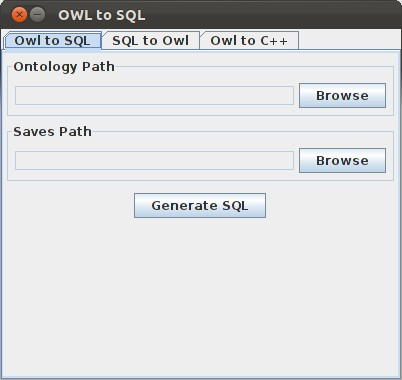
\includegraphics[width=9cm]{Figure/OWLtoSQL001.jpeg}
\caption{Owl to SQL tab.}
\label{fig:owl2sql}
\end{figure}
To convert OWL classes and instances to SQL, the \texttt{Owl to SQL} tab should be selected (see Figure~\ref{fig:owl2sql}). The different fields are:

\subsubsection{Generate SQL Files}
\begin{itemize}
 \item Ontology Path: This field requires the file \texttt{kittingInstances.owl}. Before doing so, you need to modify one line in this file. Open it with a text editor and find the line \texttt{Import(<file:kittingClasses.owl>)}. Modify
this line by giving the absolute path to the file \texttt{kittingClasses.owl}. You should should have something that looks like \texttt{Import(<file:/home/username/NIST/ipmas/Generator/kittingClasses.owl>)}. When this is done, save the file, and browse to  \texttt{kittingInstances.owl} using the ``Browse" button.
 \item Browse to the directory where you want to save the SQL files.
\end{itemize}

Once the two previous steps are done, click on ``Generate SQL''. You should receive a message confirming the generation of the SQL files: \texttt{kittingInstances.owlCreateTable.sql} and \texttt{kittingInstances.owlInsertInto.sql}. The former is used to create tables, the latter is used to populate these tables;

\subsubsection{SQL Tables and Insertions}
The next step is to create a database and to populate it.

\begin{itemize}
\item Connect to mysql using \textit{mysql -u root -p}, then enter your password. You should be in the mysql shell if this succeeded (\textit{mysql>}). 
\item Create a database: 
\begin{itemize}
\item \texttt{mysql>} \textit{CREATE DATABASE OWL;}. Here, \textit{OWL} is the name of the database (you can use a name of your choice).
\item Before performing the following commands, we need to tell MySQL which database we are planning to work with (\textit{OWL} in our case). This is done using:
\begin{itemize}
\item[] \texttt{mysql>} \textit{USE OWL}
\end{itemize} 
\end{itemize} 
\item Populate the database with tables using \texttt{kittingInstances.owlCreateTable.sql}. 
\begin{itemize}
 \item \texttt{mysql>} \textit{source <path>/kittingInstances.owlCreateTable.sql;}
\end{itemize} 
 
\item Populate the tables with data using \texttt{kittingInstances.owlInsertInto.sql}: 
\begin{itemize}
 \item \texttt{mysql>} \textit{source <path>/kittingInstances.owlInsertInto.sql;}
\end{itemize} 
\end{itemize} 

\textit{<path>} designs the absolute path to the appropriate file.

\subsection{OWL to C++}
\begin{figure}[h!t!]
\centering
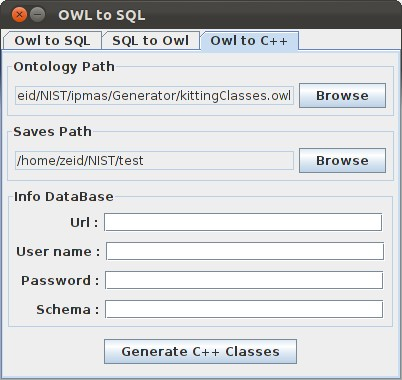
\includegraphics[width=9cm]{Figure/OWL2C++.jpeg}
\caption{Owl to C++ tab.}
\label{fig:owl2C++}
\end{figure}
The ``Owl to C++" tab (see Figure~\ref{fig:owl2C++}) is used to generate C++ classes and scripts allowing the connection between C++ and MySQL. The different fields are explained below:
\begin{itemize}
\item \textbf{Ontology Path}: This is the path to the ontology (\texttt{kittingClasses.owl} in our example). 
\item \textbf{Saves Path}: Directory where the C++ files and scripts will be generated.
\item \textbf{Url}: This is the url of the database. It's usually the IP address of the machine hosting the database (127.0.0.1 if it is local).
\item \textbf{User name}: User name used to connect to the MySQL database.
\item \textbf{Password}: Password associated to the user name to connect to the MySQL database.
\item \textbf{Schema}: This is the name of the database (\textit{OWL} in our example).
\end{itemize}

When all the fields are completed, click the ``Generate C++ Classes" button to generate C++ and script files.
\end{document}



